\documentclass[aspectratio=169,10pt]{beamer}

\usepackage[utf8]{inputenc}
\usepackage[T1]{fontenc}
\usepackage{amsmath, amssymb, bm}
\usepackage{booktabs}
\usepackage{xcolor}
\usepackage{tikz}
\usepackage{graphicx}
\usepackage{adjustbox}
\usepackage{helvet}
\usepackage{hyperref}
\usepackage{ifthen}
\usepackage{lmodern}
\usefonttheme{professionalfonts}
\renewcommand{\familydefault}{\sfdefault}

\usetikzlibrary{
  arrows.meta,
  backgrounds,
  calc,
  decorations.pathreplacing,
  positioning,
  shapes.geometric,
  shapes.symbols,
  shadows.blur
}

\definecolor{PhysicsBlue}{HTML}{1F4E79}
\definecolor{MLOrange}{HTML}{C46A1A}
\definecolor{GateGreen}{HTML}{2E7D32}
\definecolor{UnsafeRed}{HTML}{B23A3A}
\definecolor{ScopeGray}{HTML}{666666}
\definecolor{Ink}{HTML}{1F2937}
\definecolor{BlueFill}{HTML}{EDF3F8}
\definecolor{OrangeFill}{HTML}{FBF1E6}
\definecolor{GreenFill}{HTML}{EAF4EA}
\definecolor{RedFill}{HTML}{F8ECEC}
\definecolor{GrayFill}{HTML}{F2F2F2}
\definecolor{Canvas}{HTML}{FFFFFF}

\setbeamercolor{background canvas}{bg=Canvas}
\setbeamercolor{normal text}{fg=Ink}
\setbeamercolor{frametitle}{fg=Ink,bg=Canvas}
\setbeamercolor{title}{fg=Ink}
\setbeamertemplate{navigation symbols}{}
\setbeamersize{text margin left=0.45cm,text margin right=0.45cm}
\setbeamertemplate{footline}{
  \hfill
  \raisebox{0.15cm}{\color{ScopeGray}\scriptsize\insertframenumber}
  \hspace{0.35cm}
}
\setbeamertemplate{frametitle}{
  \vspace{0.18cm}
  \begin{beamercolorbox}[wd=\textwidth,sep=0pt]{frametitle}
    {\large\bfseries\insertframetitle}
  \end{beamercolorbox}
  \vspace{0.08cm}
  {\color{PhysicsBlue!60}\rule{\textwidth}{1.1pt}}
}

\newcommand{\takeaway}[1]{%
  \vspace{0.06cm}
  \begin{center}
    {\color{ScopeGray!70}\rule{0.92\linewidth}{0.45pt}}\\[-1pt]
    {\scriptsize\textbf{Takeaway:} #1}
  \end{center}
}

\newcommand{\scopefooter}[1]{%
  \begin{center}
  \begin{tikzpicture}
    \node[
      fill=GrayFill,
      rounded corners=8pt,
      inner xsep=8pt,
      inner ysep=5pt
    ] {\parbox{0.94\linewidth}{\centering\scriptsize\color{ScopeGray}#1}};
  \end{tikzpicture}
  \end{center}
}

\newcommand{\infocard}[4]{%
  \begin{tikzpicture}
    \node[
      draw=#1!35,
      fill=#2,
      rounded corners=3pt,
      line width=0.8pt,
      inner xsep=8pt,
      inner ysep=6pt
    ] {\parbox{#3}{#4}};
  \end{tikzpicture}
}

\newcommand{\dbicon}[1][1]{%
\begin{tikzpicture}[scale=#1, baseline=-0.6ex]
  \fill[PhysicsBlue!18, draw=PhysicsBlue, line width=0.9pt] (0,0.82) ellipse (0.95 and 0.26);
  \fill[BlueFill, draw=PhysicsBlue, line width=0.9pt]
    (-0.95,0.82) -- (-0.95,-0.55)
    arc (180:360:0.95 and 0.26) -- (0.95,0.82)
    arc (0:180:0.95 and 0.26);
  \draw[PhysicsBlue, line width=0.9pt] (0,0.16) ellipse (0.95 and 0.26);
  \draw[PhysicsBlue, line width=0.9pt] (0,-0.55) ellipse (0.95 and 0.26);
\end{tikzpicture}}

\newcommand{\saticon}[1][1]{%
\begin{tikzpicture}[scale=#1, baseline=-0.6ex]
  \fill[MLOrange!18, draw=MLOrange, line width=0.9pt] (-1.1,0.1) rectangle (-0.2,0.48);
  \fill[MLOrange!18, draw=MLOrange, line width=0.9pt] (0.68,0.1) rectangle (1.58,0.48);
  \fill[ScopeGray!28, draw=Ink, line width=0.9pt] (0,0) rectangle (0.48,0.58);
  \draw[Ink, line width=0.95pt] (0.24,0.58) -- (0.9,1.05);
  \fill[PhysicsBlue!18, draw=PhysicsBlue, line width=0.9pt] (0.9,1.05) circle (0.14);
  \draw[Ink, line width=0.9pt] (-0.2,0.29) -- (0,0.29);
  \draw[Ink, line width=0.9pt] (0.48,0.29) -- (0.68,0.29);
\end{tikzpicture}}

\newcommand{\earthorbiticon}[1][1]{%
\begin{tikzpicture}[scale=#1, baseline=-0.6ex]
  \fill[PhysicsBlue!18, draw=PhysicsBlue, line width=0.9pt] (0,0) circle (0.62);
  \draw[PhysicsBlue!60, line width=1.2pt] (0,0) ellipse (1.6 and 0.72);
  \draw[PhysicsBlue!35, dashed, line width=0.9pt] (0,0) ellipse (1.1 and 1.55);
  \fill[MLOrange, draw=MLOrange] (1.48,0.0) circle (0.12);
  \fill[PhysicsBlue!60] (-0.18,0.18) circle (0.12);
  \fill[PhysicsBlue!40] (0.2,-0.1) circle (0.08);
\end{tikzpicture}}

\newcommand{\nnicon}[1][1]{%
\begin{tikzpicture}[scale=#1, baseline=-0.6ex]
  \foreach \y in {0.0,0.5,1.0} \fill[OrangeFill, draw=MLOrange, line width=0.9pt] (0,\y) circle (0.12);
  \foreach \y in {0.2,0.8} \fill[OrangeFill, draw=MLOrange, line width=0.9pt] (0.92,\y) circle (0.12);
  \foreach \y in {0.0,0.5,1.0} \fill[OrangeFill, draw=MLOrange, line width=0.9pt] (1.85,\y) circle (0.12);
  \foreach \a in {0.0,0.5,1.0} \foreach \b in {0.2,0.8} \draw[MLOrange!80, line width=0.75pt] (0,\a) -- (0.92,\b);
  \foreach \a in {0.2,0.8} \foreach \b in {0.0,0.5,1.0} \draw[MLOrange!80, line width=0.75pt] (0.92,\a) -- (1.85,\b);
\end{tikzpicture}}

\newcommand{\shieldicon}[1][1]{%
\begin{tikzpicture}[scale=#1, baseline=-0.6ex]
  \fill[GreenFill, draw=GateGreen, line width=1pt]
    (0,1.0) -- (0.72,0.82) -- (0.62,0.12) -- (0.36,-0.24) -- (0.1,0.12) -- cycle;
  \draw[GateGreen, line width=1.15pt] (0.18,0.38) -- (0.31,0.22) -- (0.55,0.62);
\end{tikzpicture}}

\newcommand{\warningicon}[1][1]{%
\begin{tikzpicture}[scale=#1, baseline=-0.6ex]
  \fill[RedFill, draw=UnsafeRed, line width=1pt] (0,0) -- (0.8,1.35) -- (-0.8,1.35) -- cycle;
  \draw[UnsafeRed, line width=1.2pt] (0,0.42) -- (0,0.95);
  \fill[UnsafeRed] (0,0.2) circle (0.07);
\end{tikzpicture}}

\newcommand{\selectoricon}[1][1]{%
\begin{tikzpicture}[scale=#1, baseline=-0.6ex]
  \draw[Ink, line width=1.1pt] (0,0.45) -- (2.2,0.45);
  \draw[Ink, line width=1.1pt] (0,-0.25) -- (2.2,-0.25);
  \draw[Ink, line width=1.2pt] (0.28,0.45) -- (1.45,-0.25);
  \fill[Ink] (0.28,0.45) circle (0.08);
  \fill[Ink] (1.45,-0.25) circle (0.08);
\end{tikzpicture}}

\newcommand{\terminalicon}[1][1]{%
\begin{tikzpicture}[scale=#1, baseline=-0.6ex]
  \fill[BlueFill, draw=PhysicsBlue, line width=1pt] (0,0) rectangle (1.24,0.88);
  \draw[PhysicsBlue, line width=1.15pt] (0.62,0.88) -- (0.62,1.42);
  \draw[PhysicsBlue, line width=1.15pt] (0.62,1.42) -- (0.25,1.82);
  \draw[PhysicsBlue, line width=1.15pt] (0.62,1.42) -- (0.99,1.82);
  \draw[PhysicsBlue, line width=0.95pt] (0.62,1.42) arc (90:160:0.42);
  \draw[PhysicsBlue, line width=0.95pt] (0.62,1.42) arc (90:20:0.42);
  \draw[PhysicsBlue, line width=0.95pt] (0.62,1.42) arc (90:170:0.65);
  \draw[PhysicsBlue, line width=0.95pt] (0.62,1.42) arc (90:10:0.65);
\end{tikzpicture}}

\newcommand{\chipicon}[1][1]{%
\begin{tikzpicture}[scale=#1, baseline=-0.6ex]
  \fill[BlueFill, draw=PhysicsBlue, line width=1pt] (0,0) rectangle (1.2,1.2);
  \foreach \x in {0.18,0.42,0.66,0.9} {
    \draw[PhysicsBlue] (\x,1.2) -- (\x,1.45);
    \draw[PhysicsBlue] (\x,0) -- (\x,-0.25);
    \draw[PhysicsBlue] (0,\x) -- (-0.25,\x);
    \draw[PhysicsBlue] (1.2,\x) -- (1.45,\x);
  }
  \draw[PhysicsBlue, line width=0.95pt] (0.28,0.28) rectangle (0.92,0.92);
\end{tikzpicture}}

\newcommand{\boundaryicon}[1][1]{%
\begin{tikzpicture}[scale=#1, baseline=-0.6ex]
  \draw[ScopeGray, dashed, line width=1pt] (0,0) rectangle (1.4,1.05);
  \draw[ScopeGray, line width=1pt] (0.2,0.22) -- (1.2,0.22);
  \draw[ScopeGray, line width=1pt] (0.2,0.53) -- (1.2,0.53);
  \draw[ScopeGray, line width=1pt] (0.2,0.84) -- (0.95,0.84);
\end{tikzpicture}}

\newcommand{\boardplaceholder}[1][1]{%
\begin{tikzpicture}[scale=#1, baseline=-0.6ex]
  \fill[gray!8, draw=ScopeGray!60, rounded corners=0.14cm, line width=0.95pt] (0,0) rectangle (4.2,2.65);
  \fill[PhysicsBlue!12, draw=PhysicsBlue!55, rounded corners=0.1cm] (0.35,0.38) rectangle (2.2,2.2);
  \fill[MLOrange!14, draw=MLOrange!65, rounded corners=0.1cm] (2.45,0.68) rectangle (3.78,1.98);
  \foreach \x in {0.55,0.82,...,1.97} {
    \draw[PhysicsBlue!60] (\x,2.2) -- (\x,2.42);
    \draw[PhysicsBlue!60] (\x,0.38) -- (\x,0.16);
  }
  \foreach \x in {2.6,2.84,...,3.63} {
    \draw[MLOrange!70] (\x,1.98) -- (\x,2.18);
    \draw[MLOrange!70] (\x,0.68) -- (\x,0.48);
  }
\end{tikzpicture}}

\begin{document}

\begin{frame}[plain]
  \vspace{0.12cm}
  \begin{center}
    {\Large\bfseries Evidence-Gated Timing/Frequency Control}\\[2pt]
    {\Large\bfseries for LR-FHSS Direct-to-Satellite IoT}
  \end{center}
  \vspace{0.18cm}
  \begin{center}
    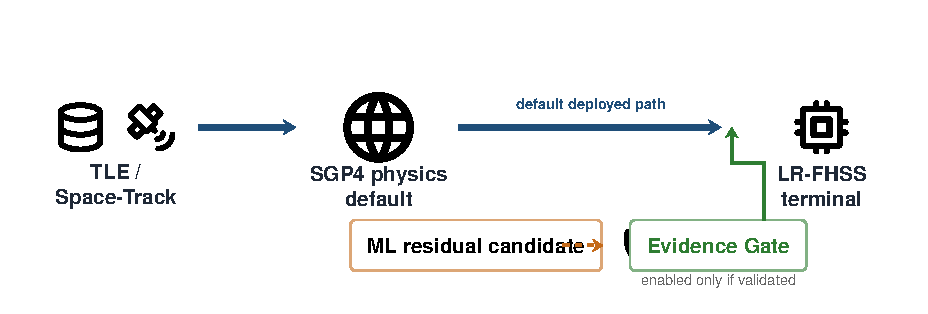
\includegraphics[width=0.96\linewidth,height=0.53\textheight,keepaspectratio]{slide_figures/fig_talk_overview.pdf}
  \end{center}
  \begin{center}
    {\large\bfseries Physics first. Evidence decides ML.}\\[2pt]
    {\scriptsize\color{ScopeGray}Software-only, model-derived study; no RF, packet, or live-satellite validation is claimed.}
  \end{center}
\end{frame}

\begin{frame}{Doppler Pre-compensation Risk}
  \begin{columns}[T,totalwidth=\textwidth]
    \column{0.24\textwidth}
    \vspace{0.42cm}
    {\small\bfseries Time-varying Doppler.}\\[0.34cm]
    {\small\bfseries Narrow LR-FHSS bins.}\\[0.34cm]
    {\small\bfseries TX window \emph{and} hop bin both uncertain.}\\[0.34cm]
    {\small\bfseries Decision before TX.}

    \column{0.76\textwidth}
    \begin{center}
      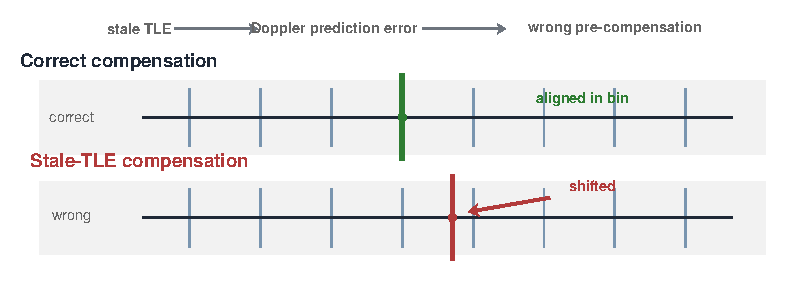
\includegraphics[width=\linewidth,height=0.68\textheight,keepaspectratio]{slide_figures/fig_hop_bin_misalignment.pdf}
    \end{center}
  \end{columns}
  \takeaway{Doppler-only is incomplete: stale orbital information is a joint timing- and frequency-control risk before transmission.}
\end{frame}

\begin{frame}{Dangerous Intuition}
  \begin{center}
    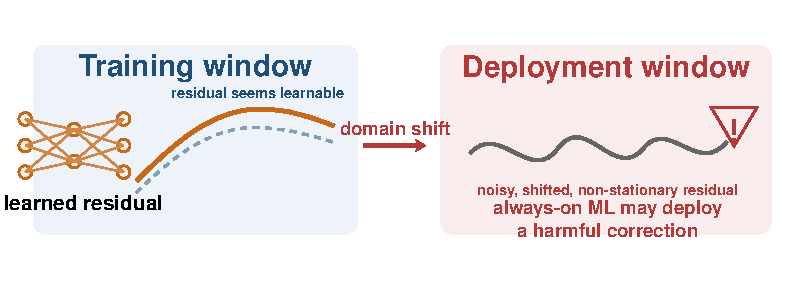
\includegraphics[width=0.98\linewidth,height=0.72\textheight,keepaspectratio]{slide_figures/fig_training_deployment_shift.pdf}
  \end{center}
  \takeaway{A learned residual is not automatically deployable.}
\end{frame}

\begin{frame}{Physics-First Framework}
  \begin{center}
    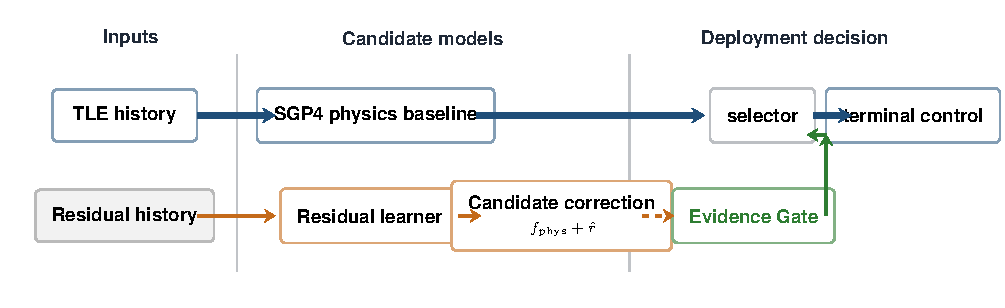
\includegraphics[width=0.99\linewidth,height=0.70\textheight,keepaspectratio]{slide_figures/fig_physics_first_architecture.pdf}
  \end{center}
  \takeaway{Physics remains connected; ML must pass through the gate.}
\end{frame}

\begin{frame}{Evidence Gate Decision Rule}
  \vspace{0.35cm}
  \begin{center}
    {\Large$\displaystyle G = \mathbf{1}\!\left[\mathrm{MAE}_{\mathrm{ML}}(V) < \gamma\,\mathrm{MAE}_{\mathrm{phys}}(V)\right]$}
  \end{center}
  \vspace{0.28cm}
  \begin{center}
    \renewcommand{\arraystretch}{1.28}
    \begin{tabular}{p{0.34\linewidth}p{0.20\linewidth}p{0.28\linewidth}}
      \toprule
      \textbf{Condition} & \textbf{Decision} & \textbf{Deployed output} \\
      \midrule
      no clear validation gain & Gate closed & SGP4 baseline \\
      validated gain & Gate open & ML correction \\
      \bottomrule
    \end{tabular}
  \end{center}
  \vspace{0.12cm}
  \begin{center}
    {\scriptsize\color{Ink!70}$V$: held-out validation window \hspace{1.5em} $\gamma$: required improvement margin}
  \end{center}
  \takeaway{If uncertain, close the gate.}
\end{frame}

\begin{frame}{Real BLACK KITE Negative Result}
  \begin{columns}[T,totalwidth=\textwidth]
    \column{0.86\textwidth}
    \begin{center}
      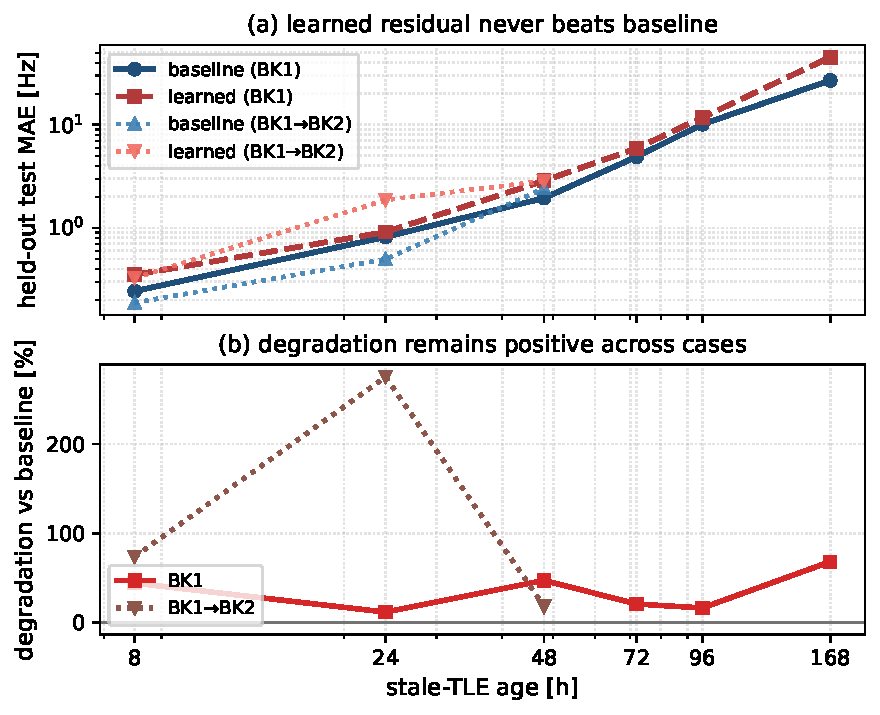
\includegraphics[width=\linewidth,height=0.80\textheight,keepaspectratio]{figures/fig_bk_residual_talk.pdf}
    \end{center}

    \column{0.14\textwidth}
    \vspace{0.92cm}
    \infocard{ScopeGray}{GrayFill}{0.84\linewidth}{\tiny
      \textbf{Result}\\
      ML residual never beats SGP4.
    }\\[0.16cm]
    \infocard{ScopeGray}{GrayFill}{0.84\linewidth}{\tiny
      \textbf{Implication}\\
      always-on ML is not justified.
    }
  \end{columns}
  \takeaway{Real BLACK KITE data does not support always-on ML.}
\end{frame}

\begin{frame}{Negative Evidence Becomes Fallback}
  \begin{center}
    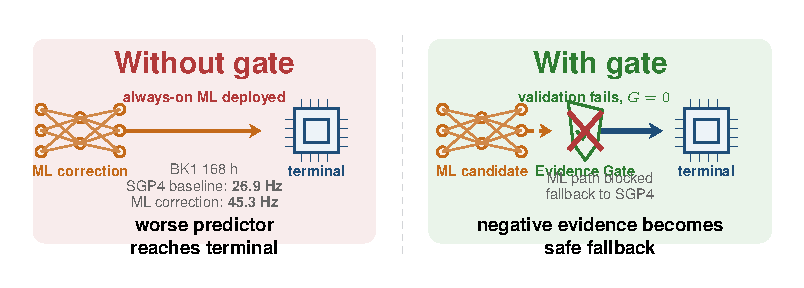
\includegraphics[width=0.98\linewidth,height=0.68\textheight,keepaspectratio]{slide_figures/fig_gate_counterfactual.pdf}
  \end{center}
  \takeaway{Negative evidence becomes a safe fallback decision.}
\end{frame}

\begin{frame}{Synthetic Sanity Check}
  \begin{columns}[T,totalwidth=\textwidth]
    \column{0.73\textwidth}
    \begin{center}
      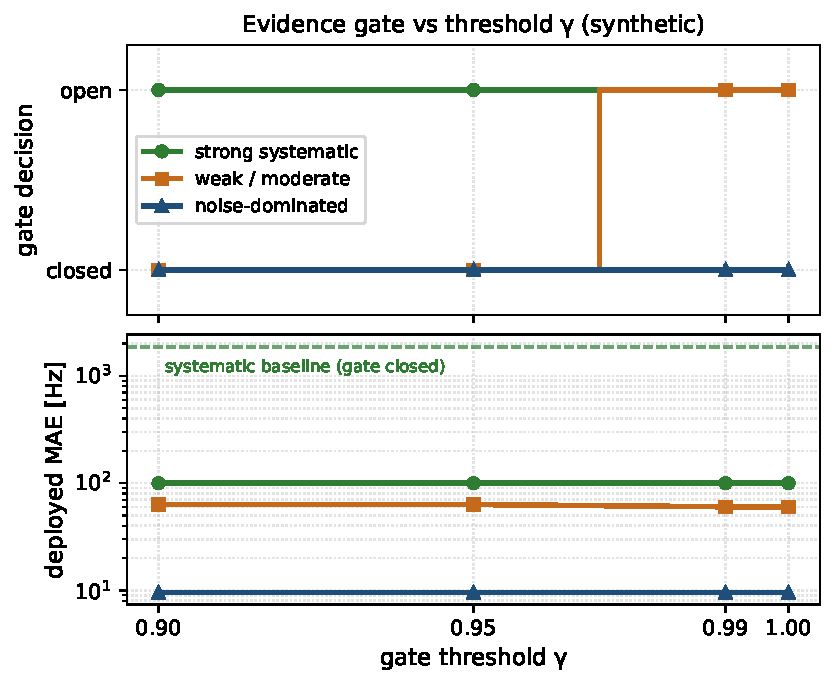
\includegraphics[width=\linewidth,height=0.72\textheight,keepaspectratio]{figures/fig_gate_behavior_talk.pdf}
    \end{center}

    \column{0.27\textwidth}
    \vspace{0.52cm}
    \renewcommand{\arraystretch}{1.18}
    \begin{tabular}{p{0.68\linewidth}p{0.20\linewidth}}
      \toprule
      \textbf{Regime} & \textbf{Gate} \\
      \midrule
      Noise-dominated & \textcolor{UnsafeRed}{closed} \\
      Weak/moderate systematic & \textcolor{UnsafeRed}{closed} \\
      Strong systematic & \textcolor{GateGreen}{open} \\
      \bottomrule
    \end{tabular}\\[0.16cm]
    {\tiny\color{ScopeGray}\parbox{0.94\linewidth}{Software-only sanity check; no hardware or live-link validation.}}
  \end{columns}
  \takeaway{The gate is conservative, not permanently closed.}
\end{frame}

\begin{frame}{Timing Sensitivity (software-only proxy)}
  \begin{center}
    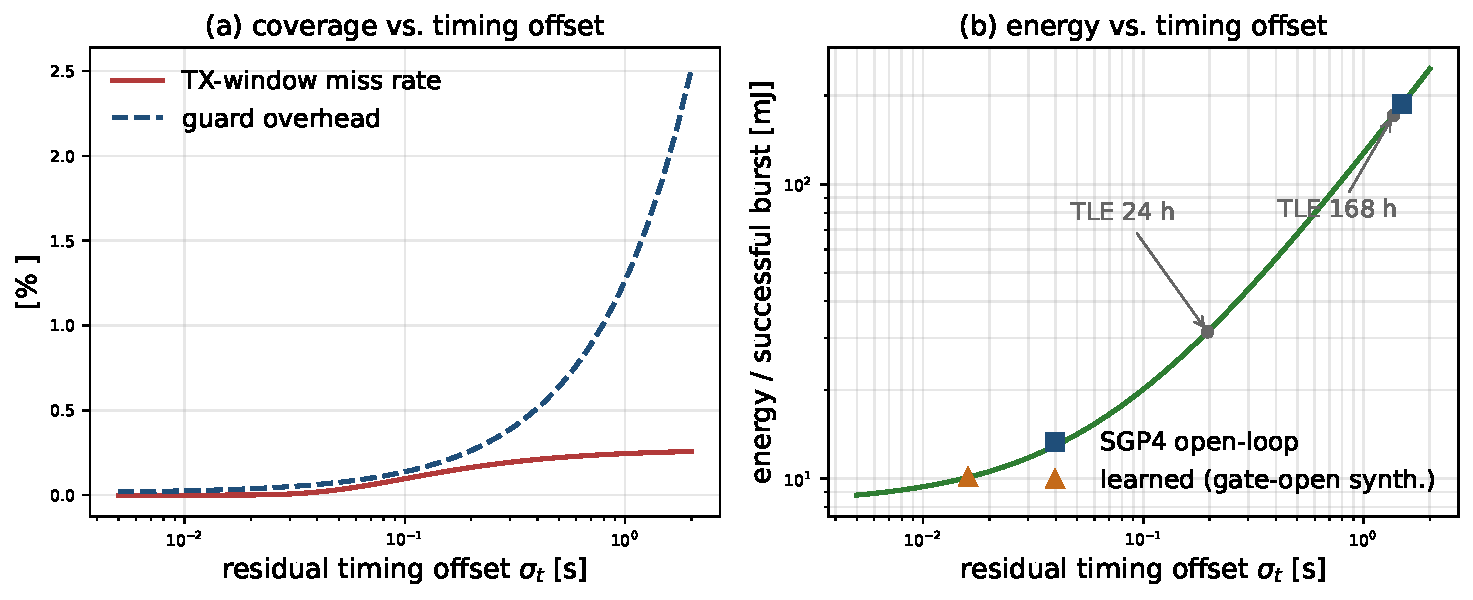
\includegraphics[width=0.90\linewidth,height=0.56\textheight,keepaspectratio]{slide_figures/fig_timing_sensitivity_talk.pdf}
  \end{center}
  \scopefooter{Guard-coverage proxy from committed \texttt{exp7} results --- analytic $\Pr[|\delta t|>g_t]$, not a measured packet outcome.}
  \takeaway{Stale-TLE timing error is paid in guard energy (${\sim}10\!\to\!{\sim}246$ mJ per successful burst), not in misses.}
\end{frame}

\begin{frame}{Timing / Frequency / PGRL Ablation (software-only proxy)}
  \begin{center}
    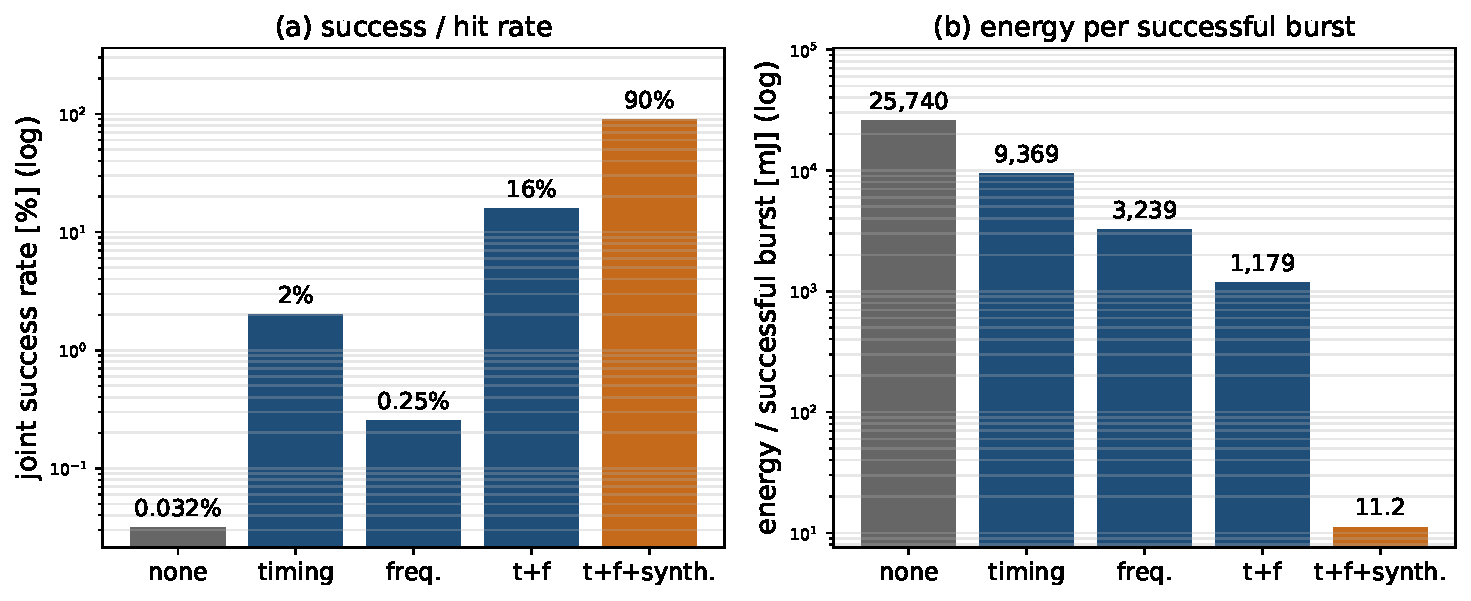
\includegraphics[width=0.90\linewidth,height=0.56\textheight,keepaspectratio]{slide_figures/fig_control_ablation_talk.pdf}
  \end{center}
  \scopefooter{Coverage proxies from committed \texttt{exp8} results. \textbf{PGRL bar = gate-open \emph{synthetic} regime}; on real BLACK KITE the gate closes.}
  \takeaway{Joint timing+frequency control moves proxy success $0.03\%\!\to\!90.4\%$, energy per success $25.7\,\mathrm{J}\!\to\!11.2$ mJ.}
\end{frame}

\begin{frame}{Conducted IQ-Level Evidence (923.2 MHz)}
  \begin{columns}[T,totalwidth=\textwidth]
    \column{0.34\textwidth}
    \vspace{0.20cm}
    \infocard{PhysicsBlue}{BlueFill}{0.94\linewidth}{\scriptsize
      \textbf{Setup}\\
      deterministic LR1121 firmware, 923.2 MHz / $-17$ dBm\\
      serial-verified: TX\_START $\to$ 39 bursts $\to$ TX\_DONE\\
      50 dB attenuated coax $\to$ USRP B210, no antenna
    }\\[0.14cm]
    \infocard{GateGreen}{GreenFill}{0.94\linewidth}{\scriptsize
      \textbf{Result}\\
      TX-ON $\mathbf{41.25\pm0.36}$ dB over TX-OFF (4 runs)\\
      2 MS/s control: 43.76 dB\\
      artifact-masked: 41.1 dB at a real hop bin\\
      before/after control: ${\sim}0.5$ dB $\to$ 41.1 dB\\
      no clipping / saturation
    }

    \column{0.66\textwidth}
    \begin{center}
      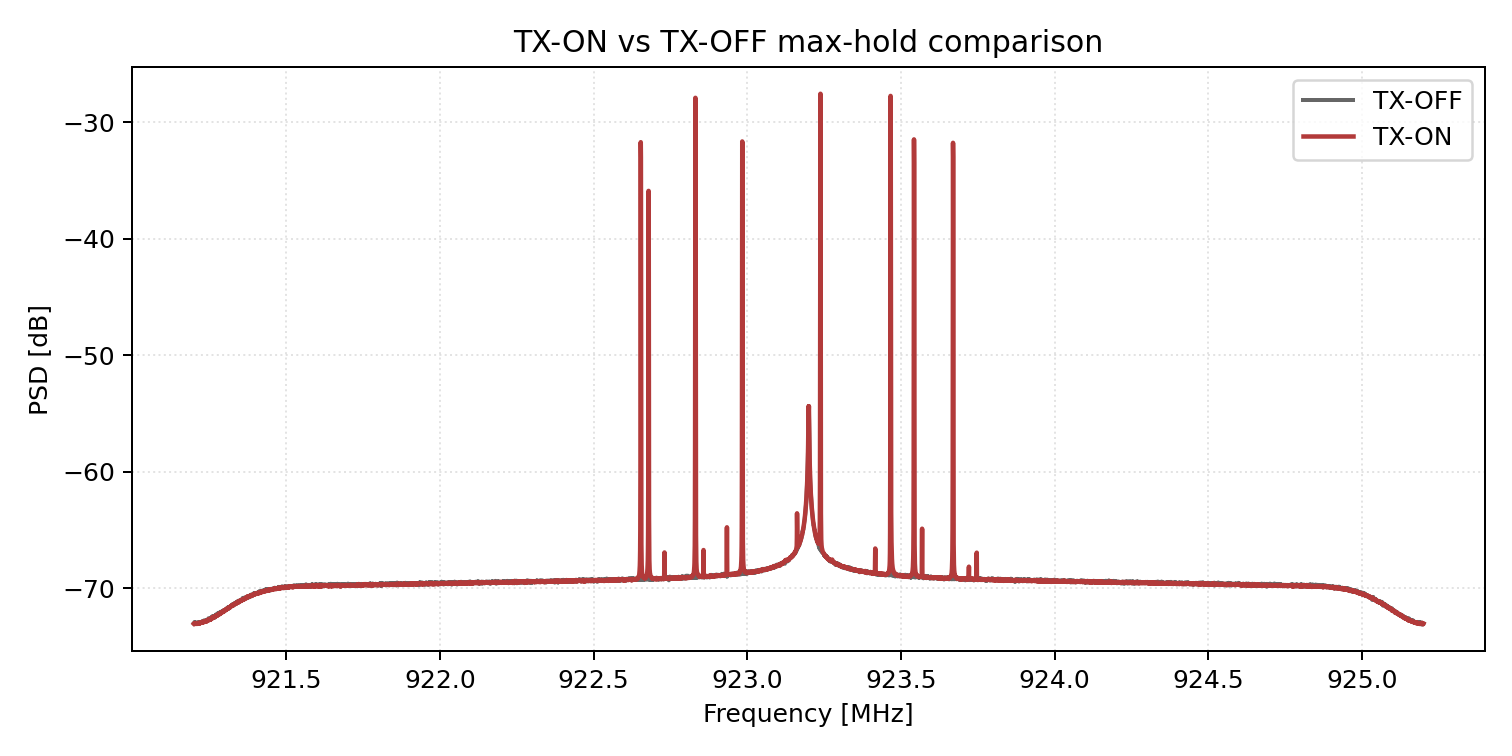
\includegraphics[width=0.99\linewidth,height=0.62\textheight,keepaspectratio]{figures_final/fig_hw_conducted_iq_txon_txoff.png}
    \end{center}
  \end{columns}
  \scopefooter{\textbf{Claim boundary:} conducted IQ-level evidence only --- no packet decoding, no PER/PDR/CRC, no gateway ACK, no OTA, no live-satellite validation.}
\end{frame}

\begin{frame}{Contributions}
  \vspace{0.22cm}
  \begin{columns}[T,totalwidth=\textwidth]
    \column{0.24\textwidth}
    \infocard{ScopeGray}{GrayFill}{0.90\linewidth}{\centering\scriptsize
      \parbox[c][2.05cm][c]{0.88\linewidth}{\centering
      
\includegraphics[height=0.34cm]{assets_external/tabler/world.pdf}\\[5pt]
      {\textbf{1. Physics-first control}}\\[-1pt]
      SGP4 remains default.}
    }

    \column{0.24\textwidth}
    \infocard{ScopeGray}{GrayFill}{0.90\linewidth}{\centering\scriptsize
      \parbox[c][2.05cm][c]{0.88\linewidth}{\centering
      
\includegraphics[height=0.34cm]{assets_external/tabler/alert-triangle.pdf}\\[5pt]
      {\textbf{2. Real-data negative result}}\\[-1pt]
      ML does not always help.}
    }

    \column{0.24\textwidth}
    \infocard{ScopeGray}{GrayFill}{0.90\linewidth}{\centering\scriptsize
      \parbox[c][2.05cm][c]{0.88\linewidth}{\centering
      
\includegraphics[height=0.34cm]{assets_external/tabler/shield-check.pdf}\\[5pt]
      {\textbf{3. Evidence-gated deployment}}\\[-1pt]
      Trust requires validation.}
    }

    \column{0.24\textwidth}
    \infocard{ScopeGray}{GrayFill}{0.90\linewidth}{\centering\scriptsize
      \parbox[c][2.05cm][c]{0.88\linewidth}{\centering
      
\includegraphics[height=0.34cm]{assets_external/tabler/cpu.pdf}\\[5pt]
      {\textbf{4. Conducted IQ-level evidence}}\\[-1pt]
      Measurement path verified; no link-layer overclaim.}
    }
  \end{columns}
  \vspace{0.52cm}
  \begin{center}
    {\Large\bfseries Do not trust ML by default.}\\[2pt]
    {\Large\bfseries Let evidence decide deployment.}
  \end{center}
\end{frame}

\end{document}
